\documentclass{amsart}

%%%%%%%%%%%%%%%

\usepackage[utf8]{inputenc}
% \usepackage[spanish]{babel}
% \usepackage[top=1in, bottom=1in, left=1.2in, right=1.2in]{geometry}
\usepackage{amssymb}
\usepackage{amsmath}
\usepackage{amsfonts}
\usepackage{amsthm}
\usepackage{wasysym}
\usepackage{enumitem}
\usepackage{graphicx}
\usepackage{listings}
\usepackage{xcolor}
\usepackage{tikz}

% sets
\newcommand{\NN}{\mathbf{N}}
\newcommand{\ZZ}{\mathbf{Z}}
\newcommand{\QQ}{\mathbf{Q}}
\newcommand{\RR}{\mathbf{R}}
\newcommand{\Zpos}{\ZZ^{+}}
\newcommand{\Rpos}{\RR^{+}}

% brackets
\newcommand{\la}{\langle}
\newcommand{\ra}{\rangle}

% formal statements
\newtheorem{prop}{Proposition}

\theoremstyle{plain}
\newtheorem{clm}{Claim}

\theoremstyle{definition}
\newtheorem{defn}{Definition}

\newtheorem{exl}{Example}

\theoremstyle{remark}
\newtheorem{rmk}{Remark}

% vulgar display of code

\lstdefinestyle{astyle}{
	commentstyle=\color{blue},
	keywordstyle=\color{purple},
	numberstyle=\tiny\color{gray},
	stringstyle=\color{green},
	basicstyle=\ttfamily\footnotesize,
	tabsize=2
}

\lstset{style=astyle}


\title{Work log of June 12 2025}
\author{Daniel R. Barrero R.}
% \date{\today}

\begin{document}

\maketitle

\section{TODOs and more}

\begin{itemize}
	\item Include Operad composition picture.
	\item Define Haskell listing manually. \texttt{<-- couldn't.}
	\item \texttt{splitForest} is a \emph{pseudoinverse} to \texttt{Cons}.
		Can't say it's an inverse because types don't match. But maybe
		that can be worked around later.
\end{itemize}

\newpage

\lstinputlisting[language=Haskell]{Operad.hs}

\newpage

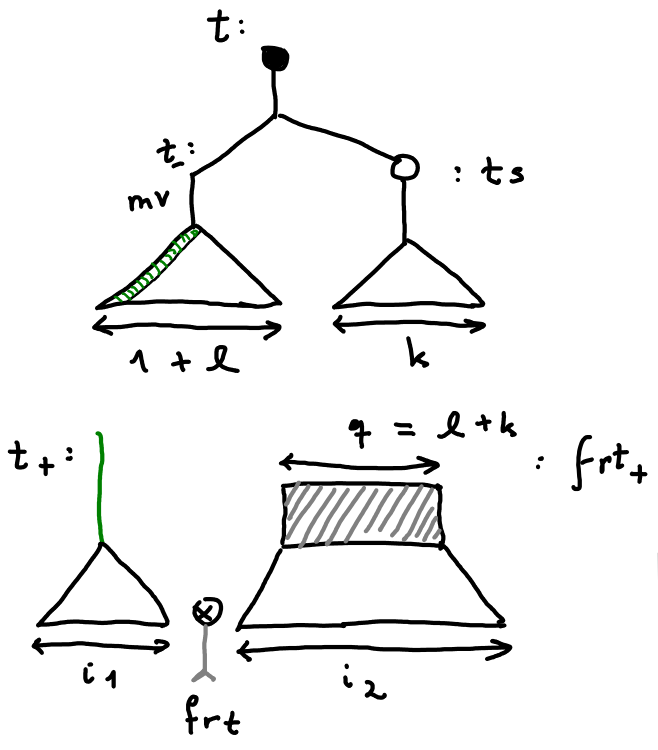
\includegraphics[width=0.7\textwidth]{bigPic.png}

\end{document}
